% =========================================================================
%  SSHVisual -- IEEE NOMS conference version (IEEEtran)
%  Converted from skeleton.tex to follow the IEEE conference template
%  (version 6/27/2024). Margins, fonts, heading styles and caption styles
%  are controlled entirely by IEEEtran.cls -- do not override them.
%  Build: pdflatex -> bibtex -> pdflatex -> pdflatex
%  Requires IEEEtran.cls and IEEEtran.bst (both ship with TeX Live / MiKTeX).
% =========================================================================

\documentclass[conference]{IEEEtran}

% ---- Packages (same set the IEEE template loads, plus what this paper uses) ----
\usepackage{cite}
\usepackage{amsmath,amssymb,amsfonts}
\usepackage{graphicx}
\usepackage{textcomp}
\usepackage{xcolor}
\usepackage{booktabs}                     % nicer table rules
\usepackage{stfloats}                     % lets figure* sit at the bottom [b] of a page
\usepackage{placeins}                     % provides \FloatBarrier

% ---- Float placement parameters (loosened so figures stay near their text) ----
\renewcommand{\topfraction}{0.9}
\renewcommand{\bottomfraction}{0.8}
\renewcommand{\textfraction}{0.07}
\renewcommand{\floatpagefraction}{0.7}
\renewcommand{\dbltopfraction}{0.9}
\renewcommand{\dblfloatpagefraction}{0.7}
\setcounter{topnumber}{3}
\setcounter{bottomnumber}{3}
\setcounter{totalnumber}{5}
\setcounter{dbltopnumber}{4}

\usepackage[hidelinks]{hyperref}          % clickable links without colored text; load last

\begin{document}

% ---- Title + Authors ----
\title{SSHVisual: Visual Tool to Analyze SSH Data}

% TODO: confirm department names and fill in email addresses or ORCIDs.
\author{\IEEEauthorblockN{Shreeman Gautam}
\IEEEauthorblockA{\textit{Kahlert School of Computing} \\
\textit{University of Utah}\\
Salt Lake City, UT, USA \\
email address or ORCID}
\and
\IEEEauthorblockN{Robert Ricci}
\IEEEauthorblockA{\textit{Kahlert School of Computing} \\
\textit{University of Utah}\\
Salt Lake City, UT, USA \\
email address or ORCID}
}

\maketitle

\begin{abstract}
Network operators use visualizations to detect attacks on their systems, interacting with data to uncover patterns that might stay hidden. Operators 
use these findings to block attackers and to expand the knowledge base of known threats. Detecting anomalies and identifying relationships iteratively in data is, 
at best, tedious and, at worst, infeasible without data visualizations. Prior work in network visualization analyzed the IP address and ASN dimensions of SSH logins with little 
focus on the username aspect of the attackers and detected anomalous network events when baseline events were available. As a result, little attention has been 
paid to whether attackers that differ in timing, source address, and username belong to the same coordinated campaign. We present SSHVisual, an iterative visualization system 
evaluated on login attacks collected from our production SSH systems. SSHVisual analyzes the IP, ASN, and username dimensions of SSH attacks, to support campaign detection. 
It complements automated detection by allowing operators to find anomalous events without a normal baseline. It uses a similarity search across dimensions that groups 
attackers by behavior and explains each match. It supports iterative and collaborative sharing of findings between operators. We evaluated SSHVisual on 
206.6 million attacker login attacks collected over 69 days. We found that it helps operators surface hidden patterns and find attackers to block. In one 
case study, some IPs tried a similar set of usernames, including uncommon ones, which pointed to a single obscure campaign that volume charts could present as unrelated 
bursts. In another, similarity search surfaced low-volume IPs working through various username lists, none of which ranked in the top ten by volume. Without similarity search, 
these IPs would likely have been hard to find and block. These results suggest that username-centric, operator-driven exploration can be valuable because it can reveal 
covertness and coordination that previous analyses can miss.

% We evaluated SSHVisual using case studies and found that it helps us block attacks
% and uncover patterns. We identified campaigns in which a set of attempted usernames recurred across unrelated IPs and ASes and we showed
% how buried some IPs are given the heavy tailed nature of SSH data.
% The similarity metric surfaced attackers returning across different time periods despite changing network origin. SSHVisual shows that treating
% usernames as a first-class analytic dimension reveals attacker coordination that IP-centric analysis misses, and that exploratory, operator-driven
% detection remains valuable.
\end{abstract}

% TODO: review keywords
\begin{IEEEkeywords}
SSH, brute-force attacks, attack campaigns, network security visualization, visual analytics, similarity search
\end{IEEEkeywords}

% =====================  I. INTRODUCTION  =====================
\section{Introduction}
\label{sec:intro}
Computer systems employ SSH \cite{ylonen1996ssh} to allow users to securely connect to them in order to execute commands and do remote
administration. Many users do a username, password combination (password based authentication) in order to gain entry to the SSH system. Attackers,
who are adversarial, can use brute force attack mechanisms \cite{295683} to get into SSH systems. Sometimes, they guess the username,
password combinations and other times, they take advantage of poorly secured systems to build botnets \cite{295683} to carry out further attacks
\cite{antonakakis2017understanding, kolias2017ddos} or steal resources from the systems, like cryptomining \cite{dang2019understanding, pastrana2019first}.

Given the prevalence of SSH attacks in the IPv4 space \cite{295683}, we designed SSHVisual and evaluated it on login attacks from our production SSH systems. 
SSHVisual serves two kinds of
network operators: Network administrators, who handle daily SSH traffic, need to identify attackers quickly and block them and Security analysts, who study traffic
over longer periods, look for patterns that are not apparent and share what they find. Consider a single period: an administrator can isolate
the highest-volume attacker and block it, while an analyst examining the same window can iteratively surface a set of low-frequency attackers that
attempt an identical sequence of usernames, and group them as a coordinated campaign.

Surveys of network visualization \cite{7166305, 6007132, zhang2017survey, raynor2022state, wu2018research} establish the maturity of the field and the gaps
we target. Our two contributions follow from treating the username, alongside the source IP and ASN, as part of an attacker’s identity, and each one 
serves one of the two operators described above. First, for security analysts, we show that username-based similarity identifies coordinated campaigns 
that volume-based views split apart. IPs that try the same list of usernames can be recognized as a single campaign, even when they come from 
different countries and ASNs and are never active on the same day. Second, for network administrators, we show that behavioral similarity
search finds attackers that may stay hidden. Operational
monitoring can focus on the largest flows ~\cite{estan2002newdirections},
and threshold detectors can be evaded by spread out attackers ~\cite{staniford2002spice,griffioen2020collaboration},
with ~\cite{gu2008botminer} showing that relationships between hosts can be found through shared behavior.
We turn this insight into a
workflow an administrator can act on: starting from a single IP they
already intend to block, our search surfaces low-volume IPs that behave
alike but could never reach the top-ten volume rankings, and it explains
each match, so the administrator knows which other IPs to block and why.



Since network traffic may not offer a stable, attack-free baseline of normal behaviour \cite{gates2006challenging}, detectors that rely on such a baseline may miss activity that doesn’t 
deviate from it in the expected way. Operators, by contrast, may recognize coordination and similarity across sessions visually, without specifying normality in advance. 
The above contributions build on this ability and are meant to complement baseline-driven detection. As operators explore, they can label and share findings 
so colleagues do not investigate the same patterns twice, and the findings can in turn inform automated detection.

The rest of the paper is as follows: Section~\ref{sec:related} is Related Work, Section~\ref{sec:tasksreqs} is Tasks and Requirements, Section~\ref{sec:design} is Design, 
Section~\ref{sec:eval} is Evaluation and Section~\ref{sec:conclusion} is Conclusion.

% =====================  II. RELATED WORK  =====================
\section{Related Work}
\label{sec:related}

A long line of visualization tools~\cite{mansmann2006interactive, oberheide2006flamingo,
mansmann2009visual, taylor2009flovis, chen2014oceans, tremel2022vitalflow,
xiao2006enhancing, goodall2009viassist, jeong2022interactive, choi2009fast}
renders network traffic and security events navigable for operators, the majority being network-flow and traffic
oriented~\cite{mansmann2006interactive, oberheide2006flamingo,
taylor2009flovis, tremel2022vitalflow, xiao2006enhancing,
jeong2022interactive, choi2009fast}, with some also integrating
intrusion-detection/prevention and host
logs~\cite{mansmann2009visual, chen2014oceans} or multidimensional
cyber-defense data~\cite{goodall2009viassist}.
Additionally, ~\cite{livnat2005visual} visualizes
IDS alerts and ~\cite{humphries2013elvis, yu2010ember} show heterogeneous security logs.
~\cite{jeong2023multi} extract
multi-resolution discrete-wavelet features from traffic, project
them with principal component analysis, and apply hierarchical clustering
across several intrusion-detection benchmarks,
separating brute-force attacks into distinct clusters.
Related work on coordinated
multiple views ~\cite{king2014coordinated, ceneda2016routingwatch, roberts2007state}
and insight generation ~\cite{yi2008understanding} informs our design.

\subsection{Username as an Actor}

To our knowledge, honeypot literature has rarely treated the username identity as an actor.
Typically, it is a dimension to count rather than to track, whereas in our analysis
it serves, alongside the IP and ASN, as an anchoring dimension. Several papers \cite{djap2021xb, visoottiviseth2011distributed, 
baykara2018novel, belqruch2019scada,
koniaris2013analysis, kyriakou2018container, koniaris2014honeypots} collect or chart honeypot traffic, with some of them
capturing SSH credentials (usernames and passwords). Where credentials are charted, like the SCADA SSH honeypot \cite{belqruch2019scada}, 
kippo-graph \cite{koniaris2013analysis},
and the container deployment \cite{kyriakou2018container}, usernames and passwords appear as static top-N tallies (kippo-graph's 
top-10 username and password bars being an example). The WAN honeypot framework 
\cite{fraunholz2017distributed} is the closest prior system 
: it computes an IP-to-IP dictionary-overlap
(containment) score to probe whether six same-/24 source IPs share a wordlist, which is a manual, one-off prototype of credential-based 
coordination analysis performed on the
IP.

\subsection{Username-Based Similarity}
Computed similarity between entities is well established in literature \cite{goodall2018situ, liao2012intelligent, pike2008putting, hao2015ensemble}. We 
do not claim similarity computation itself as novel; the contribution lies in the entity it operates on. Prior systems cluster internal hosts \cite{goodall2018situ}, 
behavioral profiles \cite{pike2008putting}, IP/port members \cite{hao2015ensemble}, or internal enterprise users
grouped by shared resources \cite{liao2012intelligent}. None treat the username as an attacker entity.
We use the username as a signature of an IP, grouping IPs by the credentials they try, with uncommon usernames weighted as stronger evidence than
ones nearly every attacker tries. Honeypot/honeynet analyses have related attack activity through time by
grouping attacks whose time series rise and fall
together~\cite{pouget2006time,thonnard2008framework}. Attackers
that share a credential list, however, need not be active
together, so we compute similarity independently of when each
attacker is active and let the operator see their time series in a linechart.

\subsection{Limits of Automated Detection}
% One premise of our approach is that SSH honeypot traffic does not admit the normal baseline that automated anomaly and campaign detection presuppose.
% The broader literature already documents the fragility of such detection: Sommer and Paxson \cite{sommer2010outside} note that machine-learning anomaly detection
% is rarely deployed for intrusion detection given the variability of ``normal,'' the cost of errors, and the difficulty of sound evaluation,
% while Axelsson \cite{axelsson2000base} shows it is throttled by the base-rate fallacy, where the false-positive rate becomes the limiting factor once
% intrusions are rare relative to benign traffic. Our setting departs from that one entirely, in the direction Gates and Taylor \cite{gates2006challenging}
% anticipate when they question whether attacks are rare or a stable normal exists, note that normal traffic may itself be malicious and malicious traffic
% unremarkable, and observe that detection ultimately devolves to an operator investigating clusters of activity by hand. The consequence is visible in the
% systems cited above: Situ \cite{goodall2018situ} learns a probabilistic model of each IP's behavior and CLIQUE \cite{best2011atypical} scores each actor
% against a baseline of its own expected activity, so both presume a per-actor ``normal'' that near-uniformly hostile, constantly churning traffic cannot supply.
% Situ nonetheless concedes that automation alone is insufficient---operators ``do not want another automated tool with algorithms they do not trust''---and
% builds a human-in-the-loop system; we reach the same conclusion from a starker starting point, lacking even the per-actor baseline it assumes, and so
% treat campaign identification as operator-driven from the outset.

Automated anomaly detection assumes a normal baseline, and SSH
traffic generally does not have one. Even where a baseline
exists, such detection is fragile.
\cite{sommer2010outside} find that machine-learning anomaly
detection is rarely deployed, because normal traffic varies
widely, errors are costly, and sound evaluation is hard.
\cite{axelsson2000base} show that when intrusions are
rare, the false-alarm rate limits any intrusion detector. Our
data is the opposite case, since nearly every login attempt is
an attack.\cite{gates2006challenging} question
whether attacks are rare and whether attack-free training data
exists at all, and note that malicious traffic can look normal.
\cite{goodall2018situ} and
\cite{best2011atypical} learn a model of each actor's
expected behavior with \cite{best2011atypical} assuming that an actor's activity
repeats weekly. However, constantly churning, near-uniformly
hostile traffic like we see cannot offer a per-actor normal. Situ also
concedes that operators ``do not want another automated tool
with algorithms they do not trust'' and keeps a human in the
loop. Lacking a per-actor baseline, we make campaign
identification operator-driven from the start.

\subsection{Username Campaigns}
% The attacks we observe do not arrive at a steady rate; they rise, fall, and change in character as events unfold in the wider world, so understanding
% them means lining them up against what is happening outside the network. The link is well documented: Bilge and Dumitras \cite{bilge2012before} found that the number of
% attacks against a given vulnerability can jump by up to five orders of magnitude -- a hundred-thousand-fold increase -- once it is publicly disclosed, and
% Sabottke et al. \cite{sabottke2015vulnerability} showed that future exploitation can be predicted from signals in disclosure channels alone. Allodi and Massacci \cite{allodi2012preliminary} add that a vulnerability's
% official severity score is a poor guide to whether it is actually attacked, so the dependable way to learn what attackers are reacting to is to watch real
% activity and line it up against real events, not to read it off a score. We want to do this at the level of a campaign -- a group of attackers acting together --
% rather than one attacker at a time, and that raises a practical problem: a campaign rarely shows up as a single source address. IP addresses do not stay tied to
% one machine -- one host is assigned many addresses over time \cite{xie2007dynamic}, hosts cycle through new addresses \cite{stone2009your}, and counting by address can overstate the number of
% real machines by orders of magnitude \cite{moura2015dynamic} -- so it is likely that a view organized by address scatters one campaign across dozens of entries that look unrelated.
% The username pulls those pieces back together: the same login names likely recur across the changing addresses, so grouping by username re-assembles the
% campaign that an address-by-address view splits apart. A username is not a perfect identity either -- names like "root" are tried by almost everyone, and
% one campaign runs through a whole list of names -- so we treat it as one analysis dimension alongside the address and the network it belongs to (its AS),
% resolving the overlaps with the similarity and grouping methods above.

We analyze attackers at the level of a campaign, meaning a group of attackers acting together, rather than one attacker at a time. That raises a 
practical problem:
a campaign rarely shows up as a single source IP. IPs may not be tied to one machine. One IP can be assigned to different hosts 
\cite{xie2007dynamic}, hosts can cycle through new IPs \cite{stone2009your}, and counting by address can overstate the number of real machines sometimes 
by an order of a magnitude
\cite{moura2015dynamic}. A view organized by address is therefore likely to scatter one campaign across dozens of entries that can look unrelated. The 
username can
pull those pieces back together. Attackers in the same campaign likely draw from a shared credential list, so the same login names 
may recur across changing IPs.
Grouping by username can reassemble the campaign that an address-by-address view could split apart.

% A username is not a perfect identity either. Names like root are tried by almost everyone, and one campaign runs through a whole list of names.
% We therefore treat the username as one analysis dimension alongside the address and the network it belongs to (its AS), not as a replacement for them.
% Uncommon usernames, which unrelated attackers are unlikely to share by chance, serve as the stronger evidence of coordination, and we resolve the remaining
% overlaps with the similarity and grouping methods described above.

\subsection{Operator Labeling and Collaboration}
The findings an operator produces can be captured and shared.
In two works \cite{guerra2019study, xiao2006enhancing}, interactive labeling was used to fold the operator's judgments back into the system. 
Collaborative analysis was
supported through shared artifacts with \cite{chen2014oceans} and \cite{goodall2009viassist} being examples. These systems establish that labeling and collaboration are valuable,
which is why our labeling-and-sharing mechanism is the step that turns an identified set of usernames into a durable, shared campaign.


% ============  III. TASKS AND REQUIREMENTS  ============
\section{Tasks and Requirements}
\label{sec:tasksreqs}

The design of SSHVisual draws on our experience as network operators and on gaps we identified in prior work on SSH attack analysis and security visualization.
From these we derive three tasks and five requirements.
% Table~\ref{tab:task-req} summarizes which requirements support which tasks.

\subsection{Tasks}
\label{sec:tasks}

\textbf{T1: Identify SSH campaigns.} Security analysts need to find attackers that behave alike across usernames, IPs, ASNs, and countries,
and record groups so they can be referenced.

\textbf{T2: Detect anomalies that warrant action.} Network administrators need to see unusual activity, like a sudden spike or a source dominating traffic,
and decide whether to block it.

\textbf{T3: Share findings across operators.} Analysts and administrators need to see what their colleagues have already investigated, so that the
same patterns are not identified twice.

\begin{figure*}[b]
  \centering
  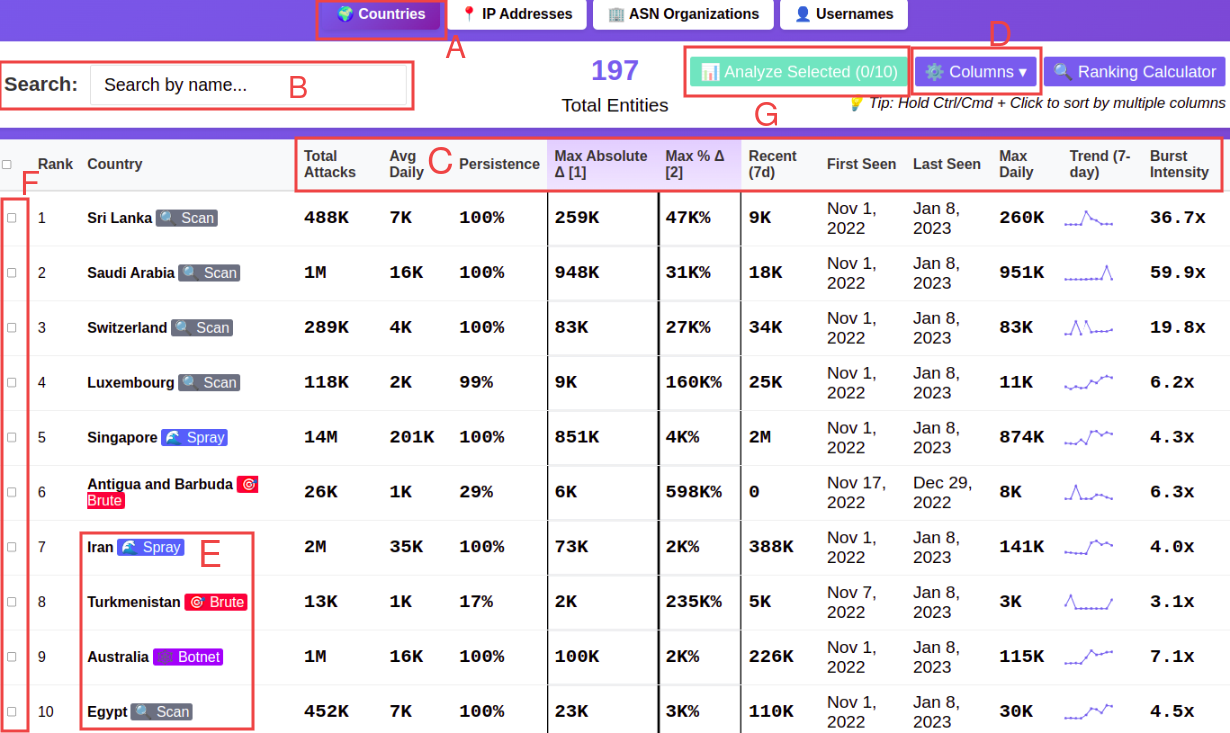
\includegraphics[width=\textwidth]{annotated-d5.png}
  \caption{Discovery table, showing the countries tab (A). Operators can filter countries(B). 
  A row shows a country and operators can sort by any mix of columns (C), with more columns present in (D). Based on attack patterns, a 
  badge is given (E). Operators can select up to 10 rows (F and G) to plot in linechart.}
  \label{fig:discovery}
\end{figure*}

\subsection{Requirements}
\label{sec:reqs}

\textbf{R1: Attacker similarity profiling.} SSHVisual should be able to cluster similar attackers along the username, IP and ASN
dimensions. R1 mostly serves T1 as it allows security analysts to build a repository of similar attackers.

\textbf{R2: Sorting and ranking.} 
SSH attack data can take many forms,
and no single view can suit them all. Two examples illustrate this.
The data can be heavy-tailed: one username can account for a
quarter of attacks~\cite{owens2008study}, and a few persistent IPs can
account for most attacks~\cite{wu2020mining}. It can also be spread out:
distributed attackers divide their attempts across many low-volume
sources, so no single entity may stand out by count.
SSHVisual should therefore list every entity in each dimension and let the operator sort
and rank entities by any combination of attributes, not only volume.
R2 supports T1 and T2: network administrators can surface anomalous
entities that never reach the top of a volume ranking, and security
analysts can rank entities by their similarity to one they are
investigating.

% \textbf{R3: Visual clarity.} Line charts become harder to read accurately as more series are added~\cite{javed2010graphical}. Each linechart should therefore show at most
% ten entities. An aggregate chart of total attacks should accompany the per-entity charts, so that operators can judge how much of the total any one entity accounts for.
% For example, if 150M attacks occur on a given day and 75M of them come from a single username, that username should stand out when the two charts are compared. R3 primarily supports T2.

\textbf{R3: Shared tagging.} Operators should be able to tag attackers, record what a tag means, and why it was applied to a particular attacker,
and have those tags remain visible to every operator. Each tag application should record who applied it and when,
so later operators can judge whether a finding is still current. R3 primarily supports T3, and supports T1 because tags accumulate into a repository of related attackers.

\textbf{R4: Complementary tabular and temporal views.} No single visualization can serve every need. A table can support precise lookup and ranking 
but can discard temporal structure;
a linechart can preserve temporal structure, showing spikes and campaigns at a glance, but can convey values less precisely ~\cite{few2006visual}. SSHVisual should 
therefore provide both views and let operators
move between them. A network administrator may find and act on an anomaly using the table alone, whereas a security analyst may use the table to assemble related attackers and
examine their behavior over time in the linecharts. R4 supports T1 and T2.

\textbf{R5: Interactive exploration of the linecharts.} The linecharts follow Shneiderman's Visual Information-Seeking Mantra: overview first, zoom and
filter, then details-on-demand~\cite{shneiderman1996eyes}. They open on the full time range, let operators zoom into a time window
and filter entities, and reveal an entity’s details on request. R5 supports T1 and T2: zooming can isolate the time window of a
suspected campaign, and filtering can remove dominant entities that would mask smaller ones. Line charts can become harder to read accurately
as more series are added~\cite{javed2010graphical}. Each linechart should therefore show few entities and we decided to cap it at 10.

% \begin{table}[t]
%   \centering
%   \caption{Mapping of requirements to tasks ($\bullet$ primary support, $\circ$ secondary support).}
%   \label{tab:task-req}
%   \begin{tabular}{lcccccc}
%     \hline
%                                 & R1        & R2        & R3        & R4        & R5        & R6        \\
%     \hline
%     T1: Identify SSH campaigns  & $\bullet$ & $\bullet$ &           & $\circ$   & $\bullet$ & $\bullet$ \\
%     T2: Detect anomalies        &           & $\bullet$ & $\bullet$ &           & $\bullet$ & $\bullet$ \\
%     T3: Share findings          &           &           &           & $\bullet$ &           &           \\
%     \hline
%   \end{tabular}
% \end{table}


% =====================  IV. DESIGN  =====================
\section{Design}
\label{sec:design}

SSHVisual combines two visual components, a discovery table and linecharts, with two non-visual components, similarity search and tagging.
Section~\ref{sec:visual} and Section~\ref{sec:nonvisual} describe them respectively. All figures show SSH login attacks
between Nov 1 2022 and Jan 8 2023, a period of 69 days.

\subsection{Visual Design}
\label{sec:visual}

SSHVisual provides two views of the data. The discovery table (Fig.~\ref{fig:discovery}) is time independent: each row summarizes one entity over time.
The linecharts (Fig.~\ref{fig:linecharts}) can be time-dependent. Both views cover the full data period by default.

\subsubsection{Discovery Table}
\label{sec:table}

% \begin{figure*}[!tb]
%   \centering
%   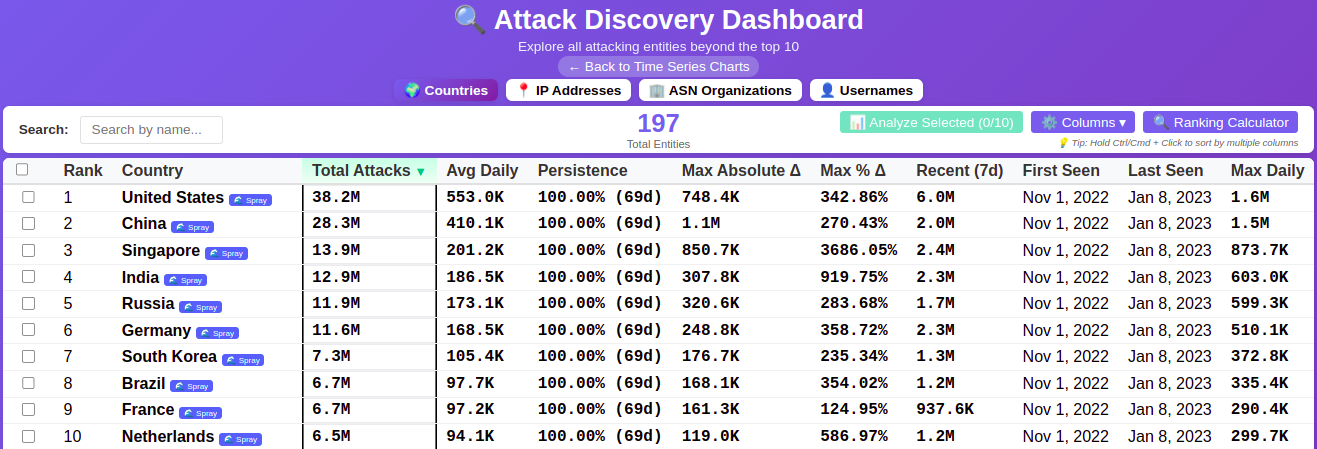
\includegraphics[width=\textwidth]{Discovery.png}
%   \caption{The discovery table, showing the countries tab. Each row summarizes one entity over the selected period, and operators can sort by any combination of columns or select up to ten rows to plot in the linecharts.}
%   \label{fig:discovery}
% \end{figure*}



The discovery table has four tabs, one per dimension: Countries, IP addresses, ASN organizations, and Usernames.
In Fig.~\ref{fig:discovery}, the Countries
tab is active (label A). A search box filters rows (label B), and the counter above the table reports the number
of entities (197 countries).
Some columns (label C) are shared across all tabs: total attacks, average daily attacks, persistence (the share of days on which the entity was active),
the largest absolute and percentage daily change, attacks in the most recent seven days, first- and last-seen dates, maximum daily count,
trend (line chart showing attacks at seven day intervals) and burst intensity (ratio of max daily attacks to average daily attacks where a higher ratio likely indicates
an entity that attacks sporadically but with higher frequencies). The full list and figures of columns (labels C and D) are found in Appendix ~\ref{app:columns}.

\begin{figure}[t]
  \centering
  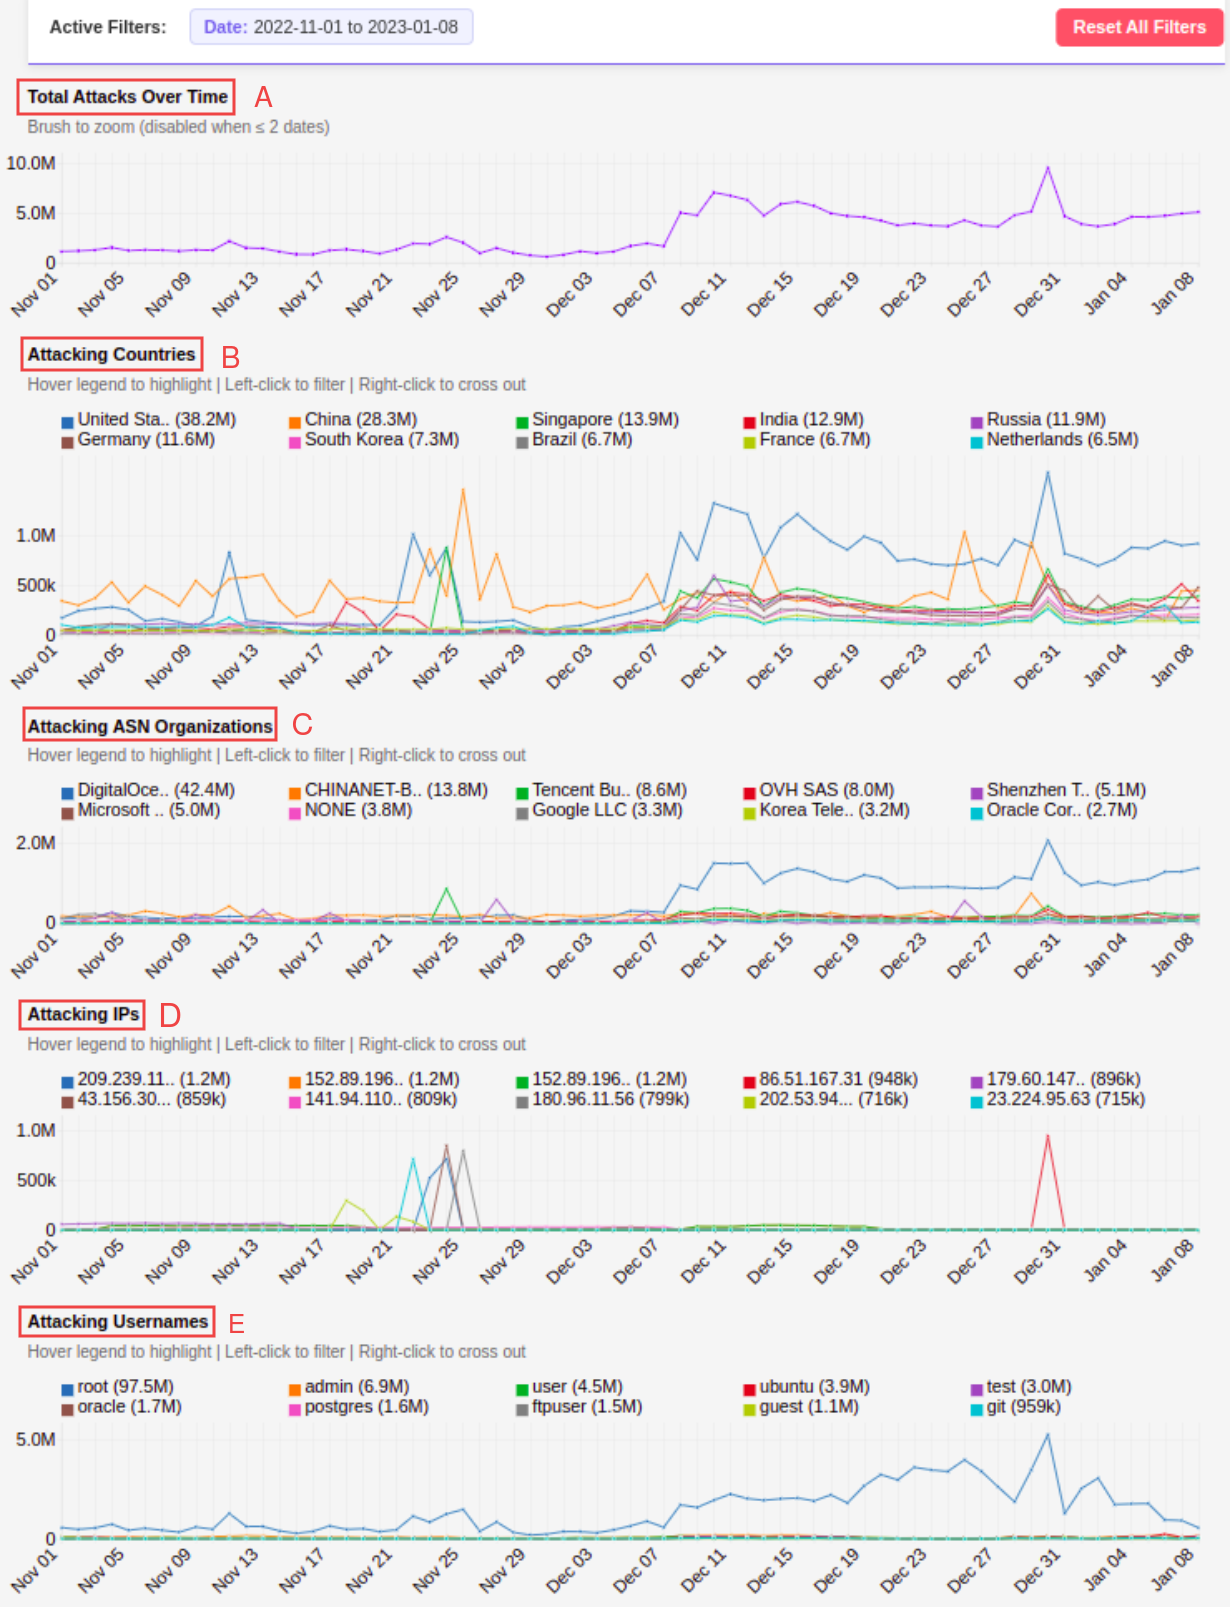
\includegraphics[width=\columnwidth]{annotated-Linechart.png}
  \caption{The top chart (A) shows total attacks over time, and the four charts below it 
  show the 10 most active countries (B), ASNs (C), IPs (D), and usernames (E). A legend entry (F) 
  identifies each series, and a brushed region (G) selects a time window. A spike appears around 
  Dec 30 (H), and two lines (I, J) follow individual countries’ attacks over time.}
  \label{fig:linecharts}
\end{figure}



Exclusive to the countries tab, each country also carries a badge summarizing its dominant behavior, namely Scan, Spray, Botnet or Brute (label E).
Brute marks entities whose traffic comes from few IP addresses making many attacks using few usernames. Spray marks traffic from many IP addresses
trying many usernames, and Botnet marks traffic spread across many IP addresses and many ASNs. Scan marks a general attack pattern that fits none
of the other three.

Unlike the linecharts, which show only the 10 most active entities per dimension, the table lists every entity. Operators can select up to 10 rows with the checkboxes (label F)
and use Analyze Selected (label G) to plot those entities in the linecharts, and they can return to the linecharts at any time. This link lets operators move from a precise,
ranked lookup to the temporal behavior of the same entities, fulfilling R4.

\begin{figure*}[t]
  \centering
  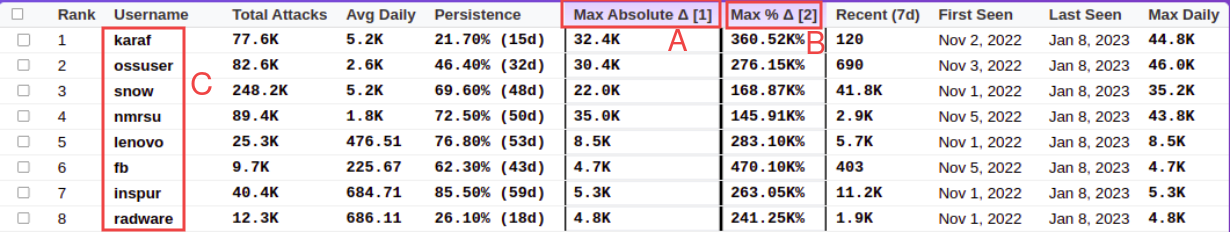
\includegraphics[width=\textwidth]{annotated-Sorting.png}
  \caption{Usernames tab sorted by Max Absolute $\Delta$ (A) and Max \% $\Delta$ (B), surfacing bursty usernames (C).}
  \label{fig:sorting}
\end{figure*}

\subsubsection{Linecharts}
\label{sec:linecharts}

% (Placed earlier in the source than its text on purpose: a full-width figure* can never appear on the page where it is defined, only on a later page.)

The linechart view (Fig.~\ref{fig:linecharts}) stacks five charts on a shared time axis. The first, Total Attacks, shows the 
aggregate volume of
attacks (label A); the remaining four show the 10 most active countries, ASNs, IPs, and usernames (labels B-E). Each legend entry (label F) lists the entity's total for the selected period.
Interaction with the linecharts follows ~\cite{shneiderman1996eyes} (fulfilling R5), and the charts are coordinated so that an action in any one of them
updates all of them.

\textbf{Overview first.} The charts cover all 69 days of data, with each chart showing the 10 most active entities in its dimension.

\textbf{Zoom.} Every chart supports brushing (label G). When the operator brushes a time range on any chart, the range is applied to all five charts and recorded in the Active Filters bar,
so the temporal context stays the same whichever dimension the operator is examining. Brushing is disabled once the range is two days or fewer, since a line needs more
datapoints.

\textbf{Filter.} Right-clicking a legend entry crosses the entity out, removing it from its chart and rescaling the y-axis so that smaller series are no longer flattened against the
axis by a dominant one. Left-clicking a legend entry selects that entity and filters every chart to the attacks associated with it. Because each attack links a username,
an IP, an ASN, and a country, the selection propagates along these relationships:

\begin{itemize}
  \item Selecting a country restricts the ASN, IP, and username charts to the entities observed in attacks from that country
  \item Selecting an ASN shows the country it originates from, along with its IPs and the usernames they try
  \item Selecting an IP shows its country and ASN, along with the usernames it tries
  \item Selecting a username shows the countries, ASNs, and IPs from which it was tried
\end{itemize}

\textbf{Details-on-demand.} Hovering over a data point shows a tooltip with that entity's attack count for the day, and hovering over a legend entry highlights the entity's line,
and the legend reports each entity's total for the selected period.

Linked filtering can turn linecharts from four separate rankings into a means of tracing an entity across dimensions. An operator investigating 
the spike on Dec 30 (label H) can select root in the username chart; the IP, ASN, and country charts then show which addresses, networks, and countries tried root, and
brushing around Dec 30 narrows the view to the spike. Conversely, selecting an ASN like DigitalOcean reveals which usernames its hosts try, indicating
whether a hosting provider’s traffic is one campaign or many. Brushing on every chart, linked filtering, and on-demand details fulfill R5.

The linecharts answer questions that the discovery table cannot, such as ``Do the countries in Fig.~\ref{fig:discovery} share the same peaks and valleys?'' or ``Does one country
begin attacking earlier than another?'' In Fig.~\ref{fig:linecharts}, the aggregate chart shows a spike on Dec 30 (label H), and most top-ten countries peak on the same
day, indicating a coordinated, multi-country event rather than a single source. The charts also reveal timing differences. China's largest peak falls in late
November (label I), weeks before the US' activity rises (label J), and the IP chart shows individual addresses that each spike for a day or two then fall silent. Neither pattern can
be recovered from the table's per-entity totals. Together, Figs.~\ref{fig:discovery} and~\ref{fig:linecharts} show how the two views complement each other, fulfilling R4.

\subsubsection{Sorting and Ranking}
\label{sec:sorting}

Fig.~\ref{fig:sorting} shows the usernames tab sorted on two columns (labels A and B). Operators sort by holding Ctrl/Cmd while clicking headers, and the bracketed
indices in the headers show when the column was clicked.

Sorting matters because the data are heavy-tailed. The username linechart in Fig.~\ref{fig:linecharts} is dominated by root,
which accounts for tens of
millions of attacks and flattens every other line. Ranking by day-over-day change instead surfaces usernames (label C in Fig.~\ref{fig:sorting}), absent from Fig.~\ref{fig:linecharts}, several of which are default accounts for specific software or hardware products (karaf, for
example, is the
default account of Apache Karaf). Their totals are far below the top ten, but their activity is concentrated: karaf was used to attack 78 thousand times,
45 thousand of them on a single day, and was active on only 15 of the 69 days. Bursts of product-specific credentials like these suggest campaigns targeting particular
devices, yet they can be invisible in a volume-ranked chart. Fig.~\ref{fig:sorting} thus shows how sorting and ranking over the full entity list fulfills R2.

% \subsubsection{Visual Clarity}
% \label{sec:clarity}
% Figure~\ref{fig:clarity} shows the upper portion of the linechart view at full size. Each per-entity chart is limited to ten series, because the accuracy with which
% people read multi-series line charts declines as the number of series grows~\cite{javed2010graphical}. Each chart has its own vertical scale, so that entities
% are legible even in dimensions with lower totals.
% The aggregate chart serves as a reference for the charts below it (R3). On 30~December the aggregate chart peaks at roughly 9.5M attempts, while the username chart
% in Figure~\ref{fig:linecharts} shows \texttt{root} at roughly 5M on the same day, so a single username accounts for about half of the spike. Comparisons across
% per-entity charts are similarly direct. The United States and DigitalOcean both rise sharply on 9~December and remain elevated for the rest of the period, and a
% spike from Singapore on 24~November coincides with a spike from Tencent in the ASN chart, consistent with attacks launched from cloud infrastructure hosted in Singapore.
% Because each chart shows at most ten lines, such correspondences can be spotted at a glance.

\subsection{Grouping and Tagging}
\label{sec:nonvisual}

The visual components help operators find individual attackers, while the grouping and tagging components help them connect those attackers
to others and record what they find. Similarity search groups attackers by behavior, in the username dimension (Section~\ref{sec:usersim})
and the IP dimension (Section~\ref{sec:ipsim}), and shared tagging (Section~\ref{sec:tagging}) preserves the resulting groups so that other
operators can build on them.

\subsubsection{Username Similarity}
\label{sec:usersim}

Similarity search lets an operator start from one username and find the
usernames that attackers use in the same way.
For usernames, the unit of analysis is the population of
sources that tries a username. For a username, we compute the breadth of that population (the number of distinct IPs, ASNs, and countries that try it),
its volume, traffic concentration on its most active source, among other features. We do not 
reuse the 17-dimensional profile we apply to
IPs (Section~\ref{sec:ipsim}), because a diagnostic showed some features to be uninformative for usernames. Daily stability is an example: 
most IPs are active many days, so their stability is well defined, but half of the usernames appear only one day, where
stability is meaningless. We cluster username profiles with k-means (k=9). Each
cluster is labeled automatically from its centroid. To answer a query, SSHVisual retrieves the query's cluster and ranks the other members by Euclidean distance to the query,
reported as a similarity score.

% its persistence,

In Fig.~\ref{fig:usersim}, an operator searches for james (label A). SSHVisual places it in Cluster~3, labeled
High-Volume Persistent Botnet-Scale,
which contains 2,624 usernames (label B). The label describes the typical username in this cluster: it
is tried in about 31,800 attacks from about 4,000 IPs, on 72\% of days.
The results table lists the 20 most similar usernames (five shown here), each with its total attacks, top country, top three source IPs,
the top three ASNs, and a set of ``Why similar?'' labels (label D), such as a
shared lead source country, comparable volume, or sourcing volume, that explain the match.

Above the results, a shared infrastructure panel (label C) lists IPs that appear as the top sources of more than one username, also shown in the
table. In Fig.~\ref{fig:usersim}, 37 IPs are shared. Each panel line names an IP and counts how many of the 100 usernames it is a
top source for, followed by examples of those usernames. Two of the most shared addresses, 152.89.196.123 and 152.89.196.220, lie in the same /24 network and
are top sources for 34 and 33 usernames respectively, including manager, daniel, and oscar. The panel applies the same analysis to ASNs: 
13 are shared, led by DigitalOcean (99 of 100 usernames), Tencent (90), and
OVH (40). This panel can turn behavioral resemblance into infrastructural
evidence: usernames tried by the same hosts are likely drawn from the same credential list and belong to the same campaign.

\begin{figure*}[t]
  \centering
  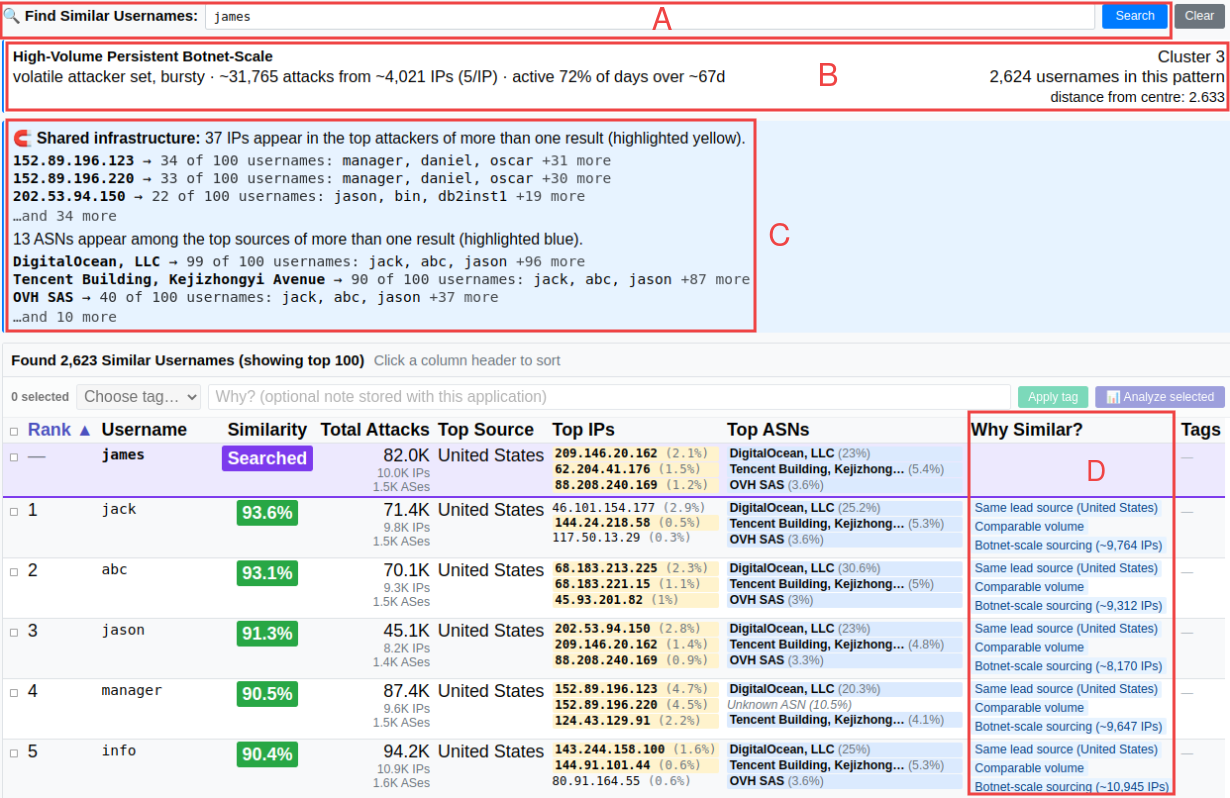
\includegraphics[width=\textwidth]{annotated-UsernameSimilarity.png}
  \caption{Similarity search for james (A). Cluster summary (B), Shared infrastructure (C), and Why similar? (D) explain why the results were grouped.}
  \label{fig:usersim}
\end{figure*}

% \begin{figure*}[!tb]
%   \centering
%   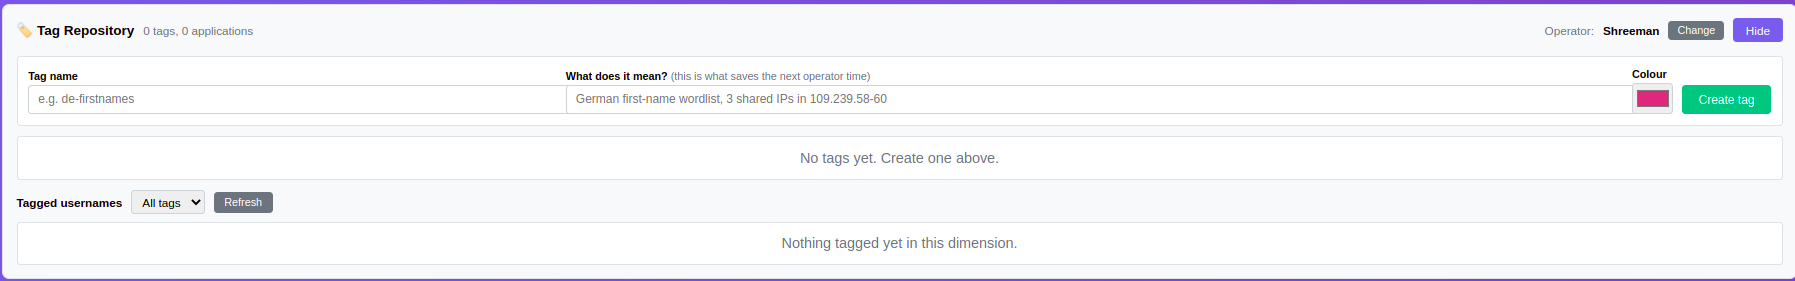
\includegraphics[width=\textwidth]{tag1.png}
%   \caption{The empty tag repository for the username dimension.}
%   \label{fig:tag1}
% \end{figure*}

\subsubsection{IP Address Similarity}
\label{sec:ipsim}

We characterize each IP address by a 17-dimensional profile drawn entirely from its activity during the data period. The features fall into four
groups: volume (log-scaled totals, daily means, and peaks); temporal shape (the fraction of days on which the address was active, its burst intensity, its 
largest daily
swings, a fitted trend slope, its activity span, and the share of its traffic in the final week); targeting behavior (unique usernames tried, how stable
that set is from one day to the next, its rotation rate, and the share of attacks taken by its most-tried username); and two flags indicating whether the address belongs to
a cloud provider and whether it originates from a major source country. We cluster these profiles with $k$-means, label each cluster
from its centroid, and answer queries in the same way as for usernames.

In Fig.~\ref{fig:ipsim}, an operator searches for 61.177.173.46 (label A), which falls in Cluster~5, labeled Low-Volume Persistent Exploratory, containing 4,405 addresses.
The most similar results are shown in label B, with similarity scores between 80.4\% and 91.2\%, all belonging to
CHINANET-BACKBONE.
Behavioral features alone can recover infrastructure relationships, suggesting that these hosts may be operated together.

Figs.~\ref{fig:usersim} and~\ref{fig:ipsim} show how SSHVisual lets operators assemble sets of similar attackers along the username and IP dimensions and see why
those attackers were grouped, fulfilling R1.

\begin{figure}[h]
  \centering
  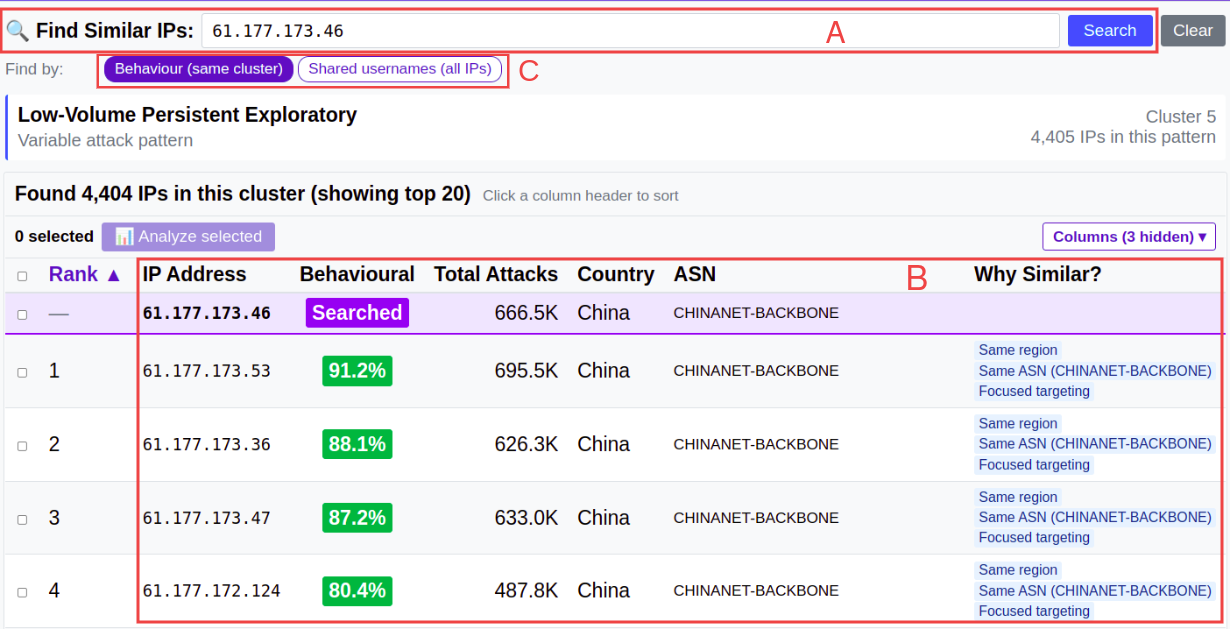
\includegraphics[width=\columnwidth]{annotated-IPSimilarity4.png}
  \caption{Similarity search (A) for IP 61.177.173.46. Nearest neighbors are adjacent addresses on the same network (B).}
  \label{fig:ipsim}
\end{figure}

\subsubsection{Shared Tagging}
\label{sec:tagging}

Figs.~\ref{fig:tag2}--\ref{fig:tag4} show how an operator records a finding so that other operators can see work that has already been done. Tags are organized in a
tag repository for each dimension. The repository displays the current operator's name, and every tag and tag application records its author.

\begin{figure}[t]
  \centering
  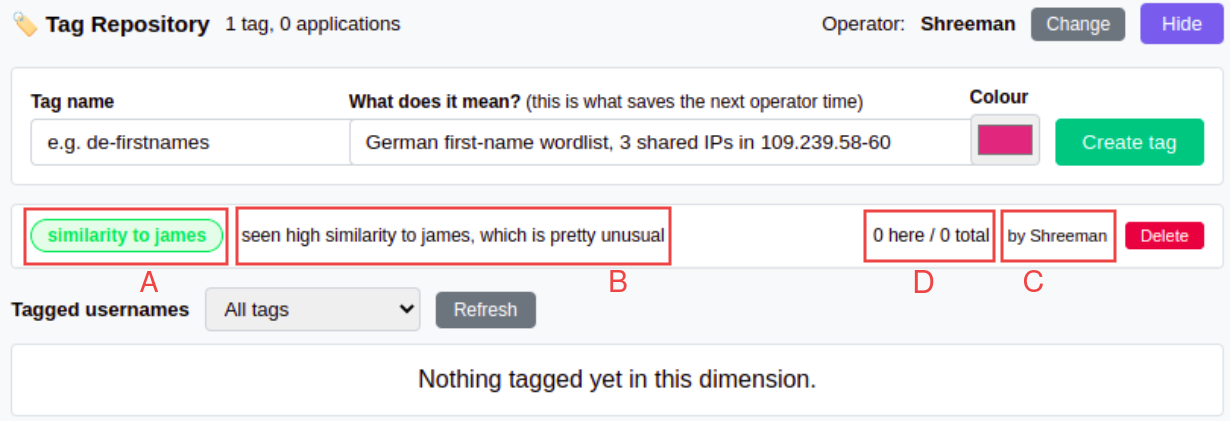
\includegraphics[width=\columnwidth]{annotated-tag21.png}
  \caption{A newly created tag (A), listed with its description (B), author (C), and application counts (D).}
  \label{fig:tag2}
\end{figure}

\begin{figure}[h]
  \centering
  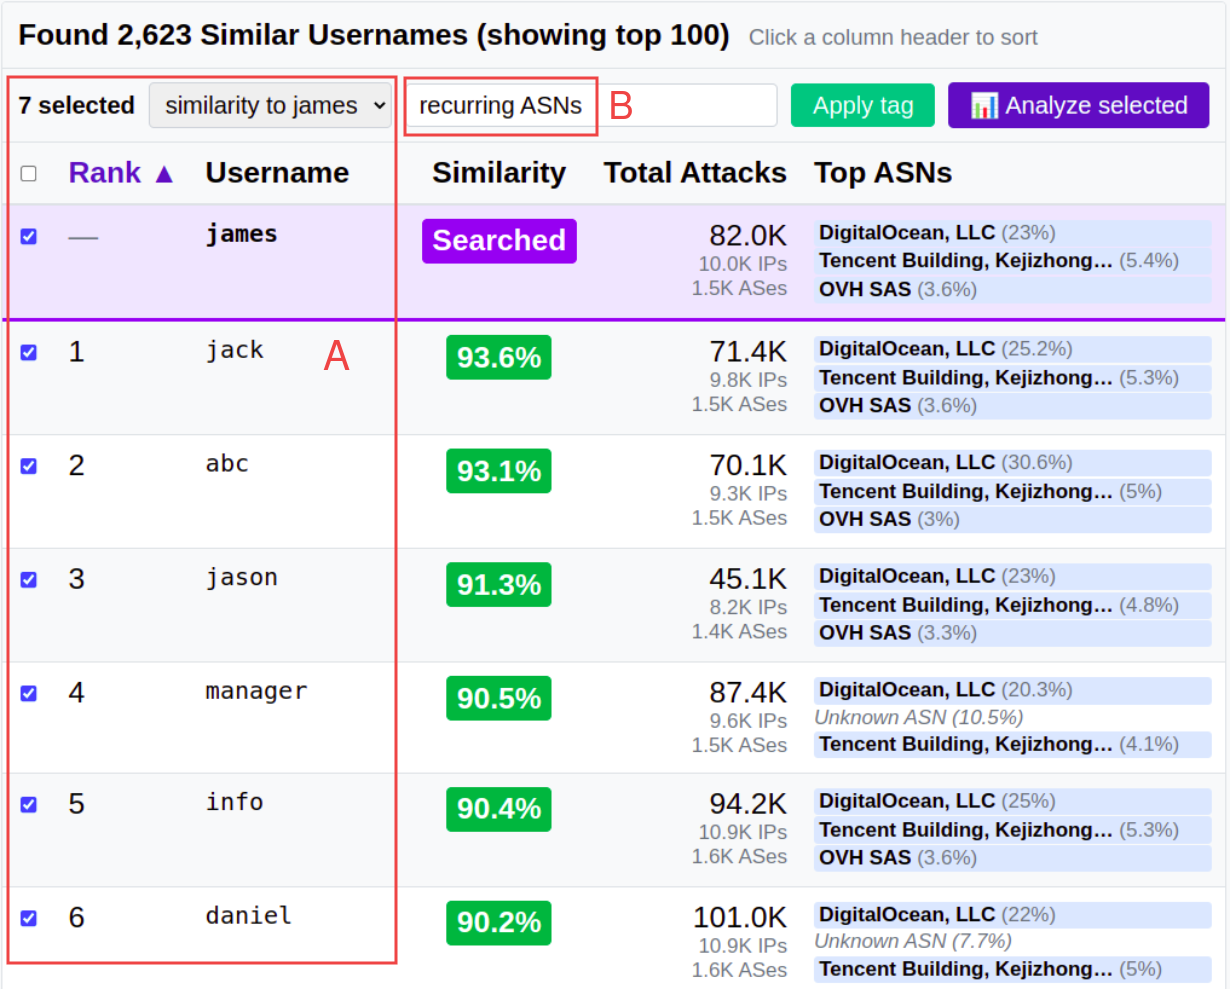
\includegraphics[width=\columnwidth]{annotated-tag31.png}
  \caption{Applying the tag to seven usernames from the similarity results (A), with a note explaining the application (B).}
  \label{fig:tag3}
\end{figure}

\begin{figure}[h]
  \centering
  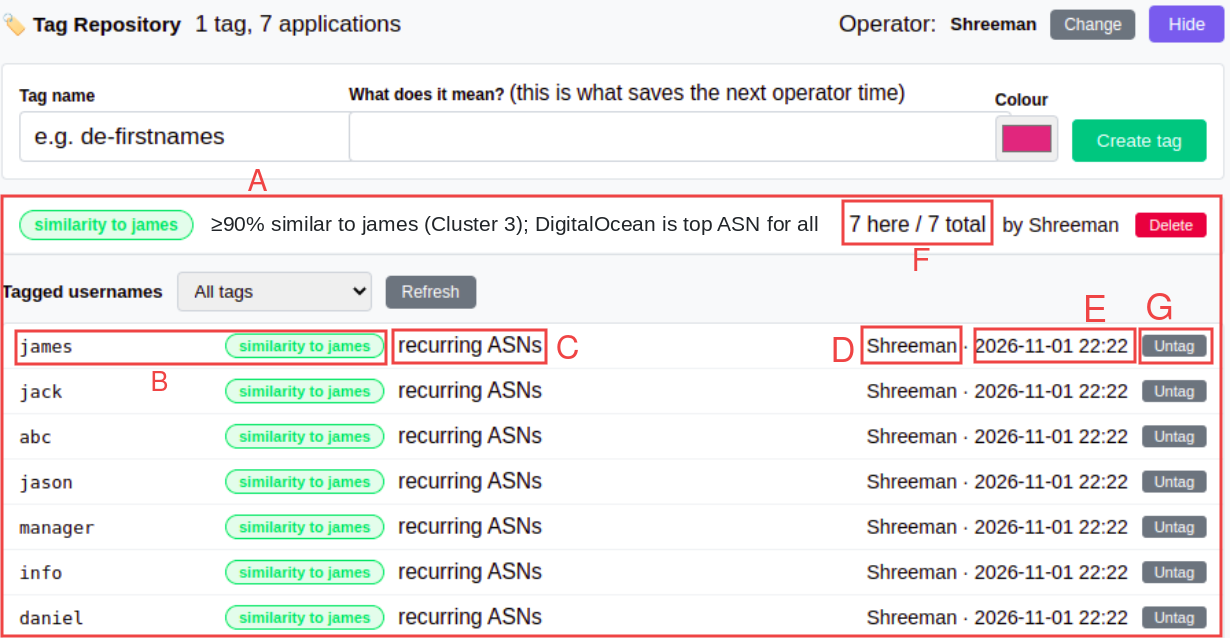
\includegraphics[width=\columnwidth]{annotated-tag43.png}
  \caption{Repository after tagging (A), listing tagged username (B) with note (C), author (D), timestamp (E), application counts (F), and untag option (G).}
  \label{fig:tag4}
\end{figure}

In Fig.~\ref{fig:tag2} the operator creates a tag, ``similarity to james'' (label A),
for the username cluster found in Fig.~\ref{fig:usersim}. The repository lists the tag with its description (label B) and its author (label C).
Tags are applied from
the similarity results. In Fig.~\ref{fig:tag3} the operator selects seven usernames (label A), chooses the
new tag, and adds a note
explaining this application: ``recurring ASNs'' (label B). In Fig.~\ref{fig:tag4} the repository reports seven applications (labels A and F).
Filtering the
list by tag shows each tagged username with its note (labels B and C), the operator who applied it (label D), and a timestamp (label E); any
application can be removed with Untag (label G).
Tagged usernames also appear in the Tags column of future similarity searches (label E in Fig.~\ref{fig:ipsim}), so an operator who later retrieves them sees immediately that
they were already investigated.
% The selection reflects the evidence from the shared infrastructure panel. All seven usernames have highlighted, shared IP addresses among their top sources, whereas
% \texttt{jack}, despite the highest similarity score, has none and is left untagged.

Separating a tag's meaning from the rationale for each application lets a later operator understand both what a group represents and why each member
belongs to it, without repeating the analysis. The recorded author and timestamp indicate whether a finding is recent. Figs.~\ref{fig:tag2}--\ref{fig:tag4}
thus show how tagging supports collaboration among operators, fulfilling R3.

\FloatBarrier % place every remaining Design figure before the next section starts

% ==============  V. EVALUATION  ==============
\section{Evaluation}
\label{sec:eval}

We evaluate SSHVisual's ability to uncover patterns and show hidden entities in two ways: 1) Security analysts finding campaigns 
in which the same usernames recur across IPs in different countries (Section~\ref{sec:sa}) and 2) Network administrators finding entities to block
that act alike but are buried underneath others (Section~\ref{sec:na}).
Both subsections start with an operator finding an IP, e.g., from an
intrusion detection alert, an abuse report, or the discovery tables in SSHVisual. On its
own, such an IP is one address among many; SSHVisual helps the operator find
what else it is connected to.

\subsection{Username Campaigns}
\label{sec:sa}

Fig.~\ref{fig:UAIPs} shows the username search (label A) for IP 68.183.213.225 (DigitalOcean, Germany). Five IPs have 100\% 
username similarity with it (labels B--F): 143.244.183.240, 24.199.108.32, and 146.190.113.228 in the US, 
134.122.62.125 in the Netherlands, and 101.204.27.20 in China. All six try the same 77 usernames, and 
every list contains all 16 of the searched IP’s uncommon usernames, such as ecell, guojing, and xxaifwq. These 
uncommon usernames make the match meaningful. A 100\% score built on common usernames like root and admin 
would say little, but 16 shared uncommon usernames are unlikely by chance. The six IPs share two ASNs 
but span four countries, consistent with a single operator renting servers in several regions. The campaign 
also extends further: at least 12 IPs score above 84\% similarity, spanning five countries and six ASNs (Appendix~\ref{app:campaigns}).

Fig.~\ref{fig:IPswoutUsernames} shows why this campaign may not be seen from volume. Each IP is active on different days: 146.190.113.228 on Dec 19 (label D), 143.244.183.240 on Dec 20 (label B), 24.199.108.32 on Dec 28 (label C),
68.183.213.225 on Jan 2 and Jan 8 (label A), 134.122.62.125 on Jan 5 to 6 (label E), and 101.204.27.20 on Nov 25 (label F). The lines never rise
together, so the chart suggests six unrelated bursts. Shared usernames can link
them into one campaign.

\begin{figure}[!tb]
\centering
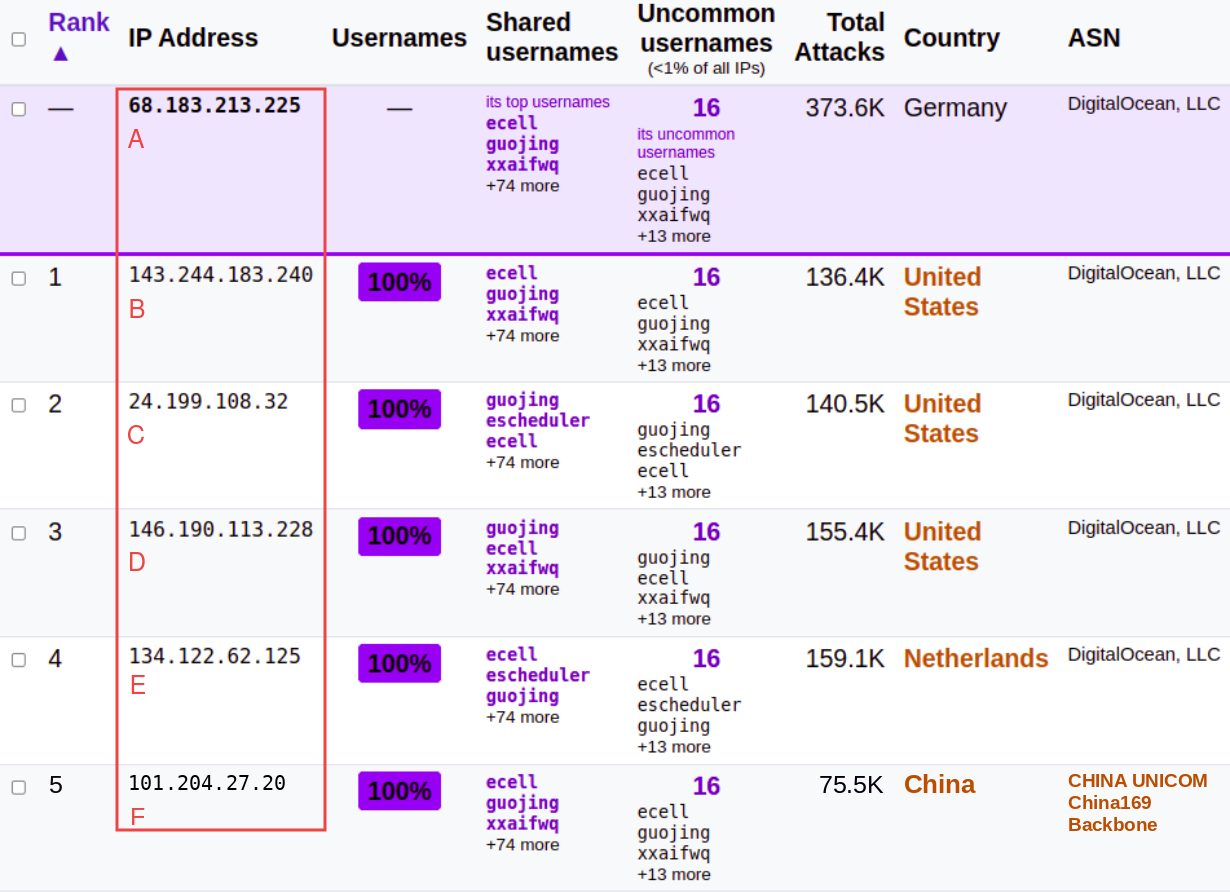
\includegraphics[width=\columnwidth]{Untitled.png}
\caption{100\% usernames shared among six IPs. IPs A, B, C, D, E, and F match the IPs A, B, C, D, E, and F in Fig.~\ref{fig:IPswoutUsernames}.}
\label{fig:UAIPs}
\end{figure}

\begin{figure}[h]
\centering
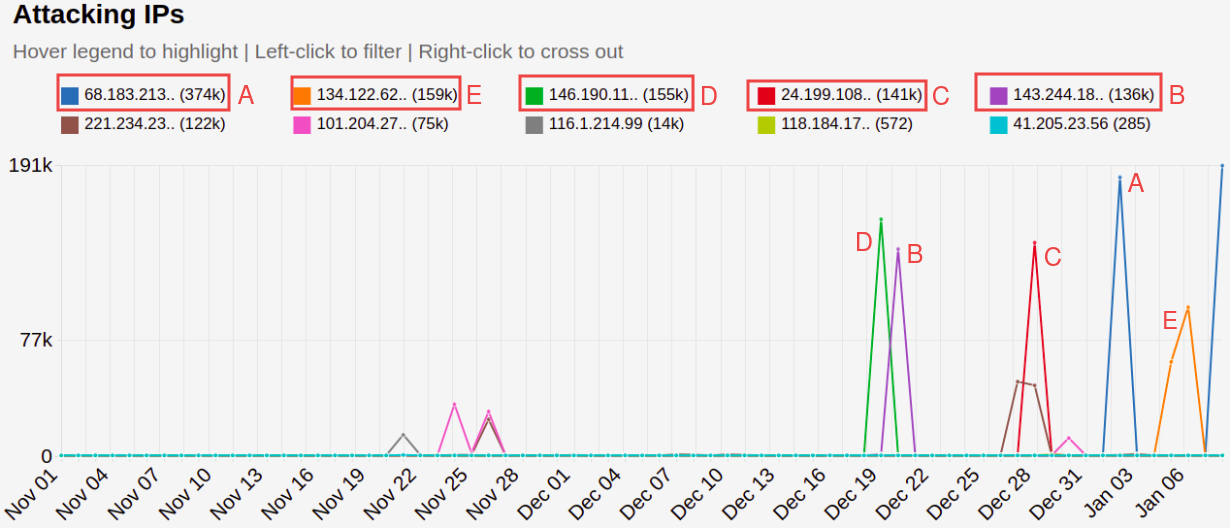
\includegraphics[width=\columnwidth]{annotated-UsernameCampaignVisual1.png}
\caption{Six IPs labeled A--F from Fig.~\ref{fig:UAIPs} in the linechart, along with other IPs with almost the same username list.}
\label{fig:IPswoutUsernames}
\end{figure}




\subsection{Finding Hidden Entities to Block}
\label{sec:na}

Fig.~\ref{fig:FindingPatterns} shows the IP similarity search for 200.195.169.59, an IP from Ligga Telecomunica\c{c}~{o}es S.A. in 
Brazil with 36 thousand attacks. Its five closest matches (88.6\% to 94.9\% similarity) come from Brazil, Indonesia, Italy, 
Mexico, and Australia, each from a different ASN. Despite this spread, they behave alike. Each made roughly 30-40 thousand attacks and is 
tagged as exploratory targeting, meaning they try many different usernames. Each shares 1,684 to 1,899 usernames with the 
searched IP, 46 to 140 of them uncommon (tried by fewer than 1\% of all IPs). The searched IP itself tried 3,821 usernames, 925 
of them uncommon. The pattern extends beyond these five: the top 20 matches, all at least 86\% similar, span 14 countries and 20 
ASNs (Appendix~\ref{app:hidden}). Together they show low-volume IPs in many countries working through large, overlapping 
lists of usernames at the same time.



Fig.~\ref{fig:BlockingBuried}
shows how buried these IPs are despite their interesting nature to administrators.
None of the 10 IPs (selected from Fig.~\ref{fig:FindingPatterns}) would appear in the top volume IPs chart.
The searched IP ranks \#296 of 86,985 IPs and accounts for 0.018\% of 206.6M attacks. Its
country, Brazil, is large enough to appear in the top 10 countries (\#8), but its ASN is 13
times too small to appear in the top 10 ASNs, and the IP itself is 20 times too small to
appear in the top 10 IPs. The other IPs rank between \#222 and \#2,826. An administrator
looking only at the high volume charts would see Brazil but never these IPs. With SSHVisual, administrators
know not just the IP they found to block but also similar IPs that they should block, and most importantly, why they should block them.

\begin{figure}[t]
\centering
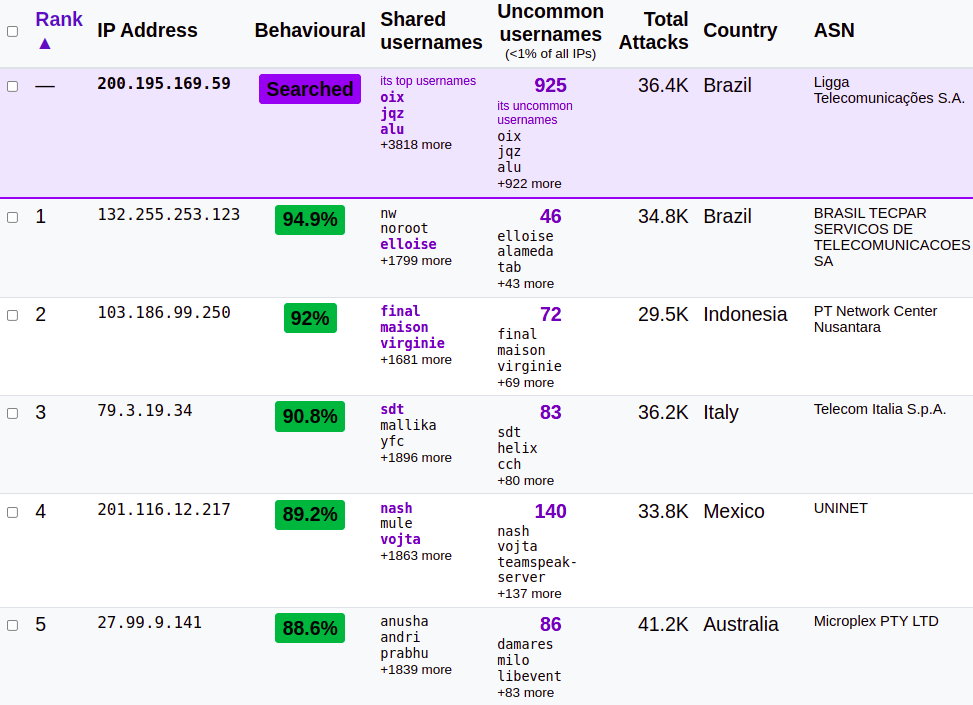
\includegraphics[width=\columnwidth]{Findingpatterns5.png}
\caption{Five IPs that behave like 200.195.169.59.}
\label{fig:FindingPatterns}
\end{figure}

\begin{figure}[t]
\centering
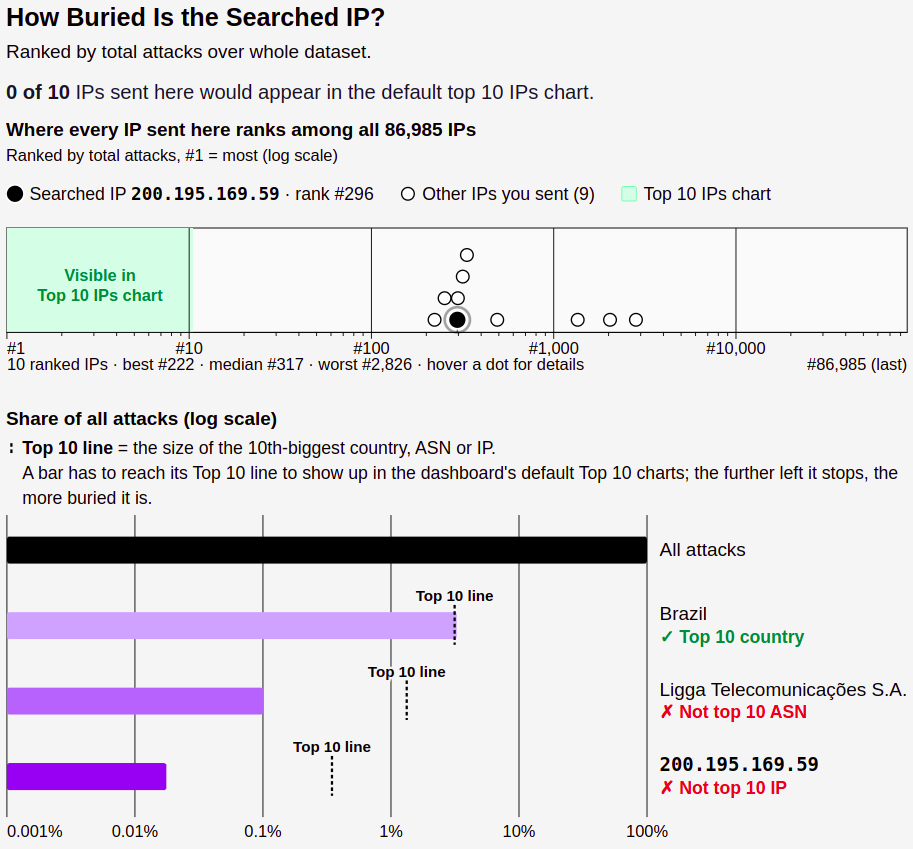
\includegraphics[width=\columnwidth]{Blockingsomethingburied1.png}
\caption{How buried 200.195.169.59 and its similar IPs are.}
\label{fig:BlockingBuried}
\end{figure}

% =====================  VI. CONCLUSION  =====================
\section{Conclusion}
\label{sec:conclusion}

We presented SSHVisual, a visual analytics system that treats the username as a first-class analytic dimension alongside
the IP, and ASN in SSH attack data. SSHVisual pairs a discovery table that ranks every entity with
coordinated linecharts that follow Shneiderman's mantra, so operators can move between precise lookup and temporal behavior.
Similarity search groups attackers by behavior along the username and IP dimensions and explains each match. Shared tagging
preserves those groups so that findings persist and remain visible across operators. Our case studies show that this combination
surfaces patterns that volume-based, IP-centric views can miss. Low-volume IPs can spread across many countries and ASNs worked through
similar lists of uncommon usernames, yet none ranked high enough to appear in any top-ten chart. IPs that never attacked on the
same day were linked into a single campaign only by the 77 usernames they shared. Because SSH traffic may not offer a normal
baseline for automated detection, these results suggest that exploratory, operator-driven analysis remains a necessary complement
to automated methods, and that the username is a valuable lens for recognizing coordinated attackers.

\FloatBarrier

% =====================  APPENDICES  =====================
% \appendices (IEEEtran) starts the appendix part: each \section after it is
% titled "Appendix A", "Appendix B", ... For a single, unlettered appendix,
% replace \appendices with \appendix and use \section*{Appendix}.


% \section{Second Appendix Title}
% \label{app:second}
% Add further appendices here; each becomes Appendix B, C, ...



% ---- References ----
% IEEEtran.bst = official IEEE reference style (numbered, order of first citation).
% Build: pdflatex -> bibtex -> pdflatex -> pdflatex
\bibliographystyle{IEEEtran}
\bibliography{refs}

\FloatBarrier

\appendices

\section{Discovery Table Columns}
\label{app:columns}

This appendix lists every column of the discovery table described in
Section~\ref{sec:table}. That section shows the Countries tab
(Fig.~\ref{fig:discovery}) and describes only the columns shared by all
four tabs (label C). The remaining columns are selected from the drop-down
menu (label D) and depend on the tab. Table~\ref{tab:columns} lists every
column and the tabs in which it appears, and
Figs.~\ref{fig:countries}--\ref{fig:Usernames} show all columns of the
Countries, IP Addresses, ASN Organizations, and Usernames tabs, respectively.

\textbf{Columns shared by all tabs.} The upper part of
Table~\ref{tab:columns} lists the ten columns described in
Section~\ref{sec:table}: total attacks, average daily attacks,
persistence, the largest absolute and percentage daily change, attacks in
the most recent seven days, first- and last-seen dates, maximum daily
count, trend, and burst intensity.

\textbf{Cross-dimension columns.} The lower part of
Table~\ref{tab:columns} lists columns that describe an entity in terms of
another dimension. For each of the four dimensions (usernames, IPs, ASNs,
and countries), a tab can have three such columns:
\begin{itemize}
  \item \emph{Unique count}: the number of distinct values of that
  dimension associated with the entity, e.g., how many distinct usernames
  a country's IPs tried.
  \item \emph{Stability}: the mean Jaccard similarity between consecutive
  days' sets of that dimension, from 0 (volatile) to 1 (stable). A higher
  value means the entity uses the same values from day to day.
  \item \emph{Concentration}: the top three values of that dimension and
  their percentages of the entity's attacks.
\end{itemize}
A tab never has these columns for its own dimension; for example, the
Usernames tab has no username stability column. The IP tab also has no ASN
or country columns of this kind, because each IP address is assumed to
belong to exactly one ASN and one country.

\begin{table}[!htb]
  \centering
  \caption{Discovery Table Columns by Tab}
  \label{tab:columns}
  \begin{tabular}{@{}lcccc@{}}
    \toprule
    \textbf{Column} & \textbf{Countries} & \textbf{IPs} & \textbf{ASNs} & \textbf{Usernames} \\
    \midrule
    Total attacks                  & $\checkmark$ & $\checkmark$ & $\checkmark$ & $\checkmark$ \\
    Average daily                  & $\checkmark$ & $\checkmark$ & $\checkmark$ & $\checkmark$ \\
    Persistence                    & $\checkmark$ & $\checkmark$ & $\checkmark$ & $\checkmark$ \\
    Max absolute $\Delta$          & $\checkmark$ & $\checkmark$ & $\checkmark$ & $\checkmark$ \\
    Max \% $\Delta$                & $\checkmark$ & $\checkmark$ & $\checkmark$ & $\checkmark$ \\
    Recent (7d)                    & $\checkmark$ & $\checkmark$ & $\checkmark$ & $\checkmark$ \\
    First / last seen              & $\checkmark$ & $\checkmark$ & $\checkmark$ & $\checkmark$ \\
    Max daily                      & $\checkmark$ & $\checkmark$ & $\checkmark$ & $\checkmark$ \\
    Trend                          & $\checkmark$ & $\checkmark$ & $\checkmark$ & $\checkmark$ \\
    Burst intensity                & $\checkmark$ & $\checkmark$ & $\checkmark$ & $\checkmark$ \\
    \midrule
    Unique usernames               & $\checkmark$ & $\checkmark$ & $\checkmark$ &              \\
    Unique IPs                     & $\checkmark$ &              & $\checkmark$ & $\checkmark$ \\
    Unique ASNs                    & $\checkmark$ &              &              & $\checkmark$ \\
    Unique Countries               &              &              &              & $\checkmark$ \\
    Username stability             & $\checkmark$ & $\checkmark$ & $\checkmark$ &              \\
    IP stability                   & $\checkmark$ &              & $\checkmark$ & $\checkmark$ \\
    ASN stability                  & $\checkmark$ &              &              & $\checkmark$ \\
    Country stability              &              &              & $\checkmark$ & $\checkmark$ \\
    Username concentration         & $\checkmark$ & $\checkmark$ & $\checkmark$ &              \\
    IP concentration               & $\checkmark$ &              & $\checkmark$ & $\checkmark$ \\
    ASN concentration              & $\checkmark$ &              &              & $\checkmark$ \\
    Country concentration          &              &              & $\checkmark$ & $\checkmark$ \\
    \bottomrule
  \end{tabular}
\end{table}


\begin{figure*}[t]
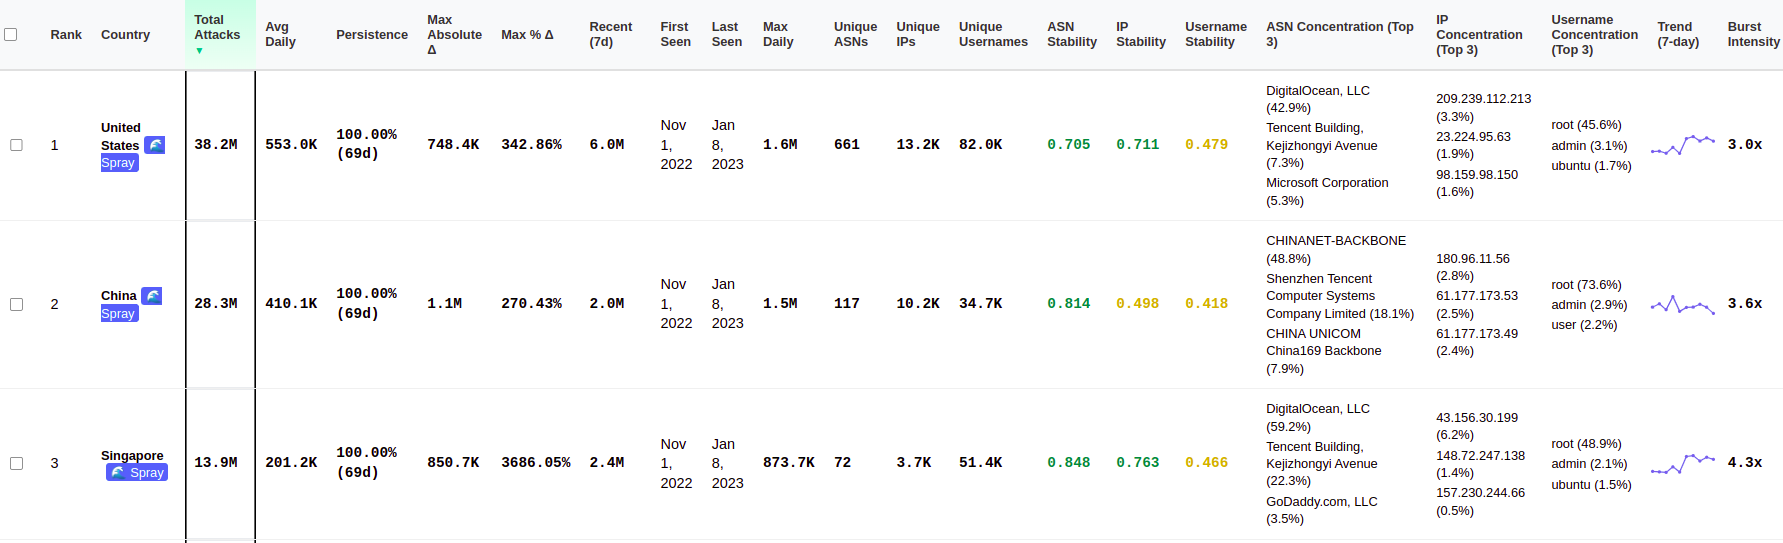
\includegraphics[width=\textwidth]{A1.png}
\caption{All the columns of the Countries tab}
\label{fig:countries}
\end{figure*}

\begin{figure*}[t]
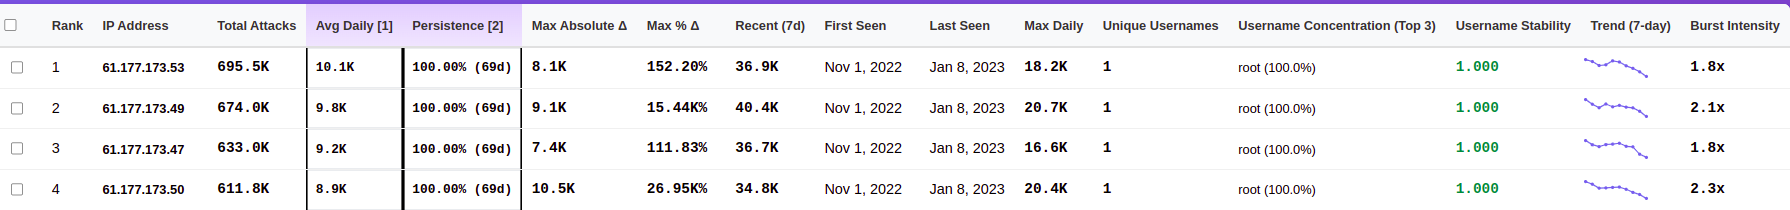
\includegraphics[width=\textwidth]{A2.png}
\caption{All the columns of the IP Addresses tab}
\label{fig:IPs}
\end{figure*}

\begin{figure*}[t]
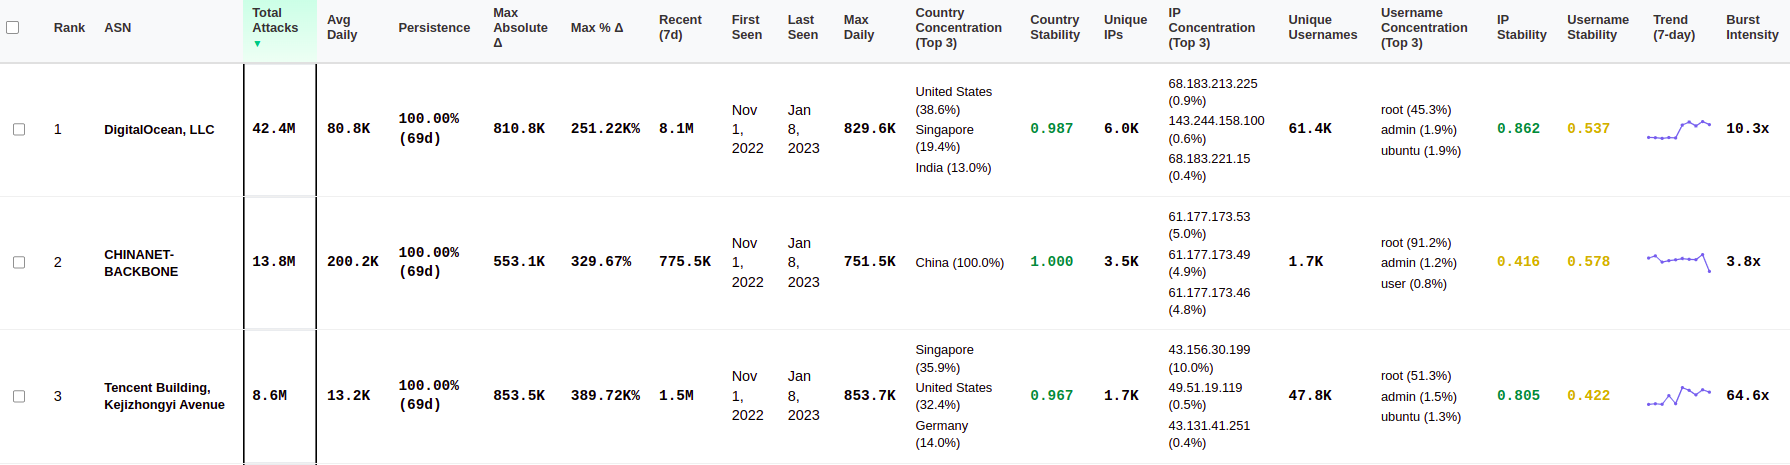
\includegraphics[width=\textwidth]{A3.png}
\caption{All the columns of the ASN Organizations tab}
\label{fig:ASNs}
\end{figure*}

\begin{figure*}[t]
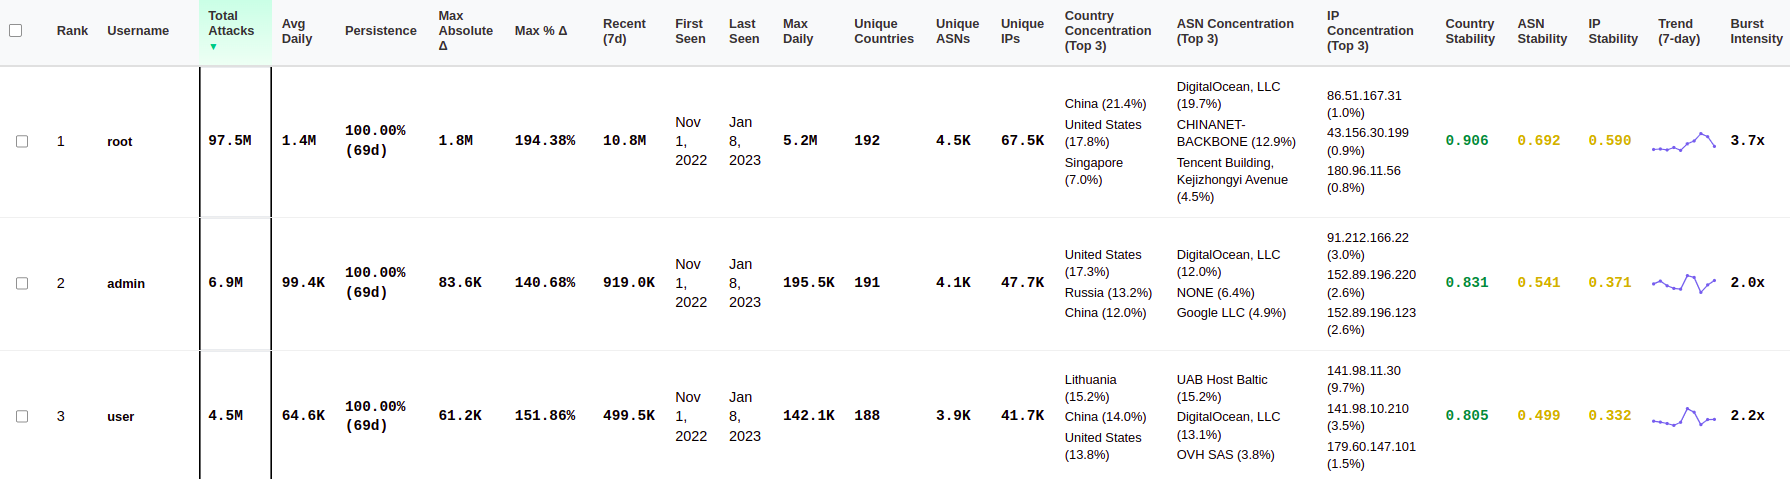
\includegraphics[width=\textwidth]{A4.png}
\caption{All the columns of the Usernames tab}
\label{fig:Usernames}
\end{figure*}


\section{Username Campaigns}
\label{app:campaigns}

This appendix extends the username campaign in Section~\ref{sec:sa}.
There, the username similarity search for 68.183.213.225 (DigitalOcean,
Germany) returned five IPs with 100\% username similarity (Fig.~\ref{fig:UAIPs}).
All six IPs tried the same 77 usernames, including 16 uncommon ones.
Fig.~\ref{fig:campaign222} shows the same search beyond those six results.
12 IPs score above 84\% similarity, and they span five countries
and six ASNs. The 100\% matches (except one) all share one ASN, but the wider set reaches
other providers. This suggests that the campaign's username list is used
beyond a single hosting provider, either by one operator renting servers
from several providers or by several operators sharing a list.

\begin{figure}[t]
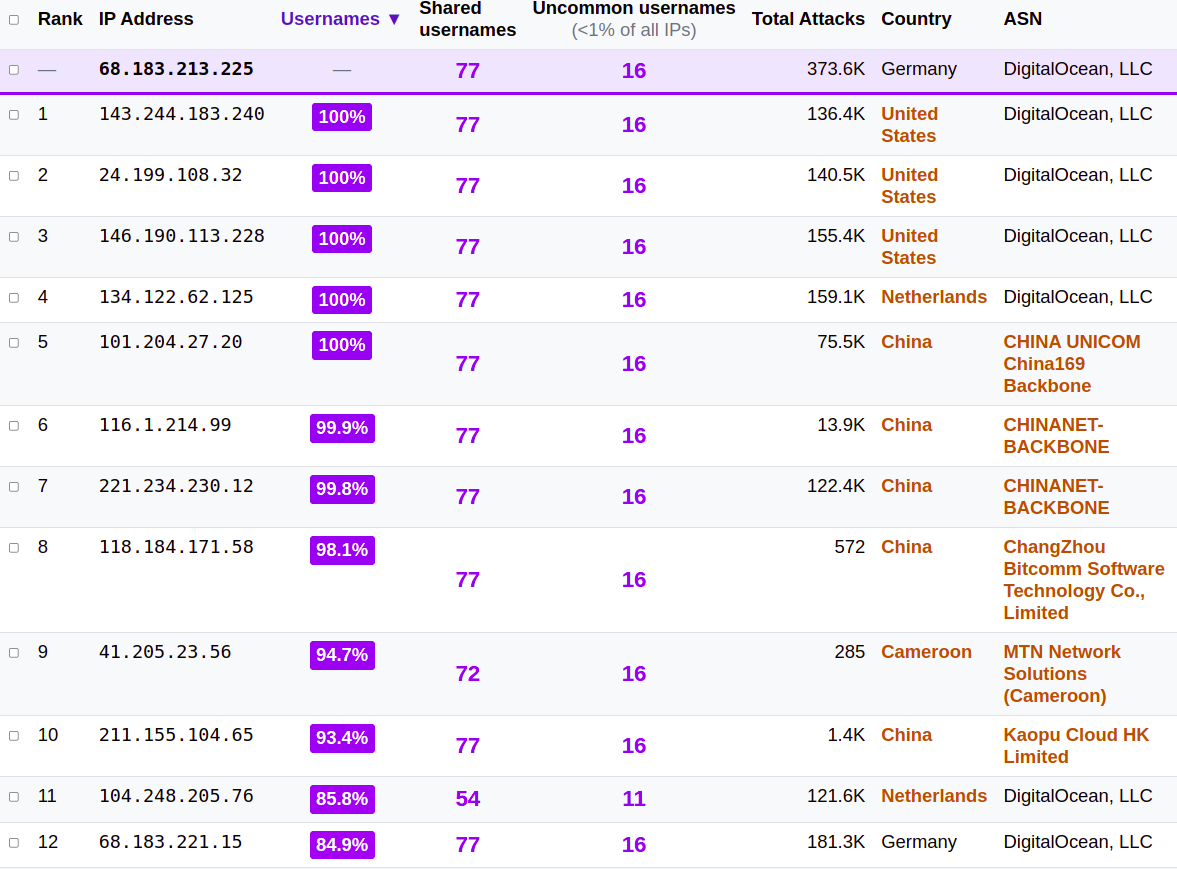
\includegraphics[width=\columnwidth]{A5.png}
\caption{Username similarity search for 68.183.213.225 (Section~\ref{sec:sa}),
showing IPs above 84\% similarity across five countries and six ASNs.}
\label{fig:campaign222}
\end{figure}


\section{Hidden Entities}
\label{app:hidden}

This appendix extends the IP similarity search in Section~\ref{sec:na}.
There, the five closest matches to 200.195.169.59 (Ligga
Telecomunica\c{c}\~{o}es S.A., Brazil) were each at least 88.6\% similar
and each came from a different country and ASN (Fig.~\ref{fig:FindingPatterns}).
Fig.~\ref{fig:campaign333} shows the top 20 matches. All are at least
86\% similar, and they span 14 countries and 20 ASNs, so no two matches
share an ASN. Blocking by country or by ASN would therefore not catch this
group. The similarity search gives
administrators the full set of IPs to block, along with the shared
behavior that justifies blocking them.

\begin{figure}[t]
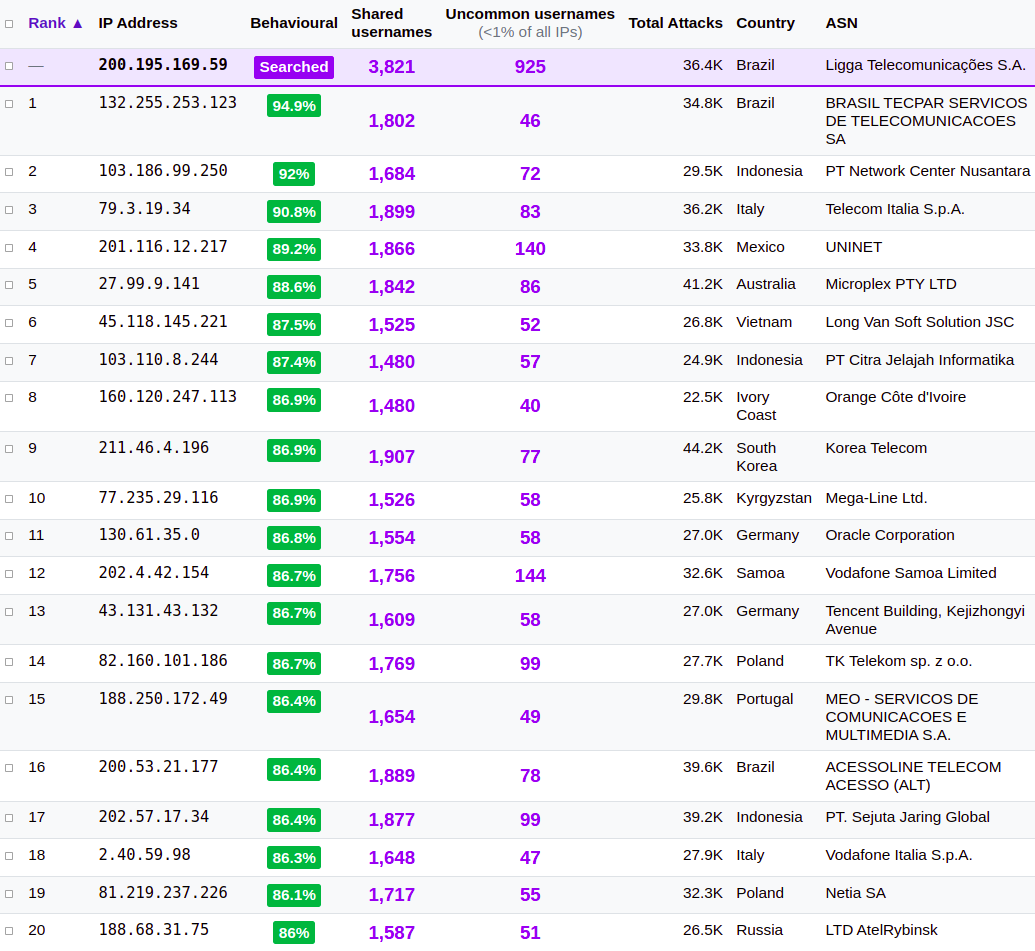
\includegraphics[width=\columnwidth]{A6.png}
\caption{Top 20 IP similarity matches for 200.195.169.59
(Section~\ref{sec:na}), spanning 14 countries and 20 ASNs.}
\label{fig:campaign333}
\end{figure}

\end{document}